\section{Diseño de PCB}

\subsection{Documentación pertinente del PCB diseñado}

A continuación, se presenta la documentación gráfica e inventario correspondientes a la placa de circuito impreso (PCB) diseñada en Altium Designer para implementar el sistema de muestreo.

\subsubsection{Esquematico.}
\begin{figure}[H]
	\centering
	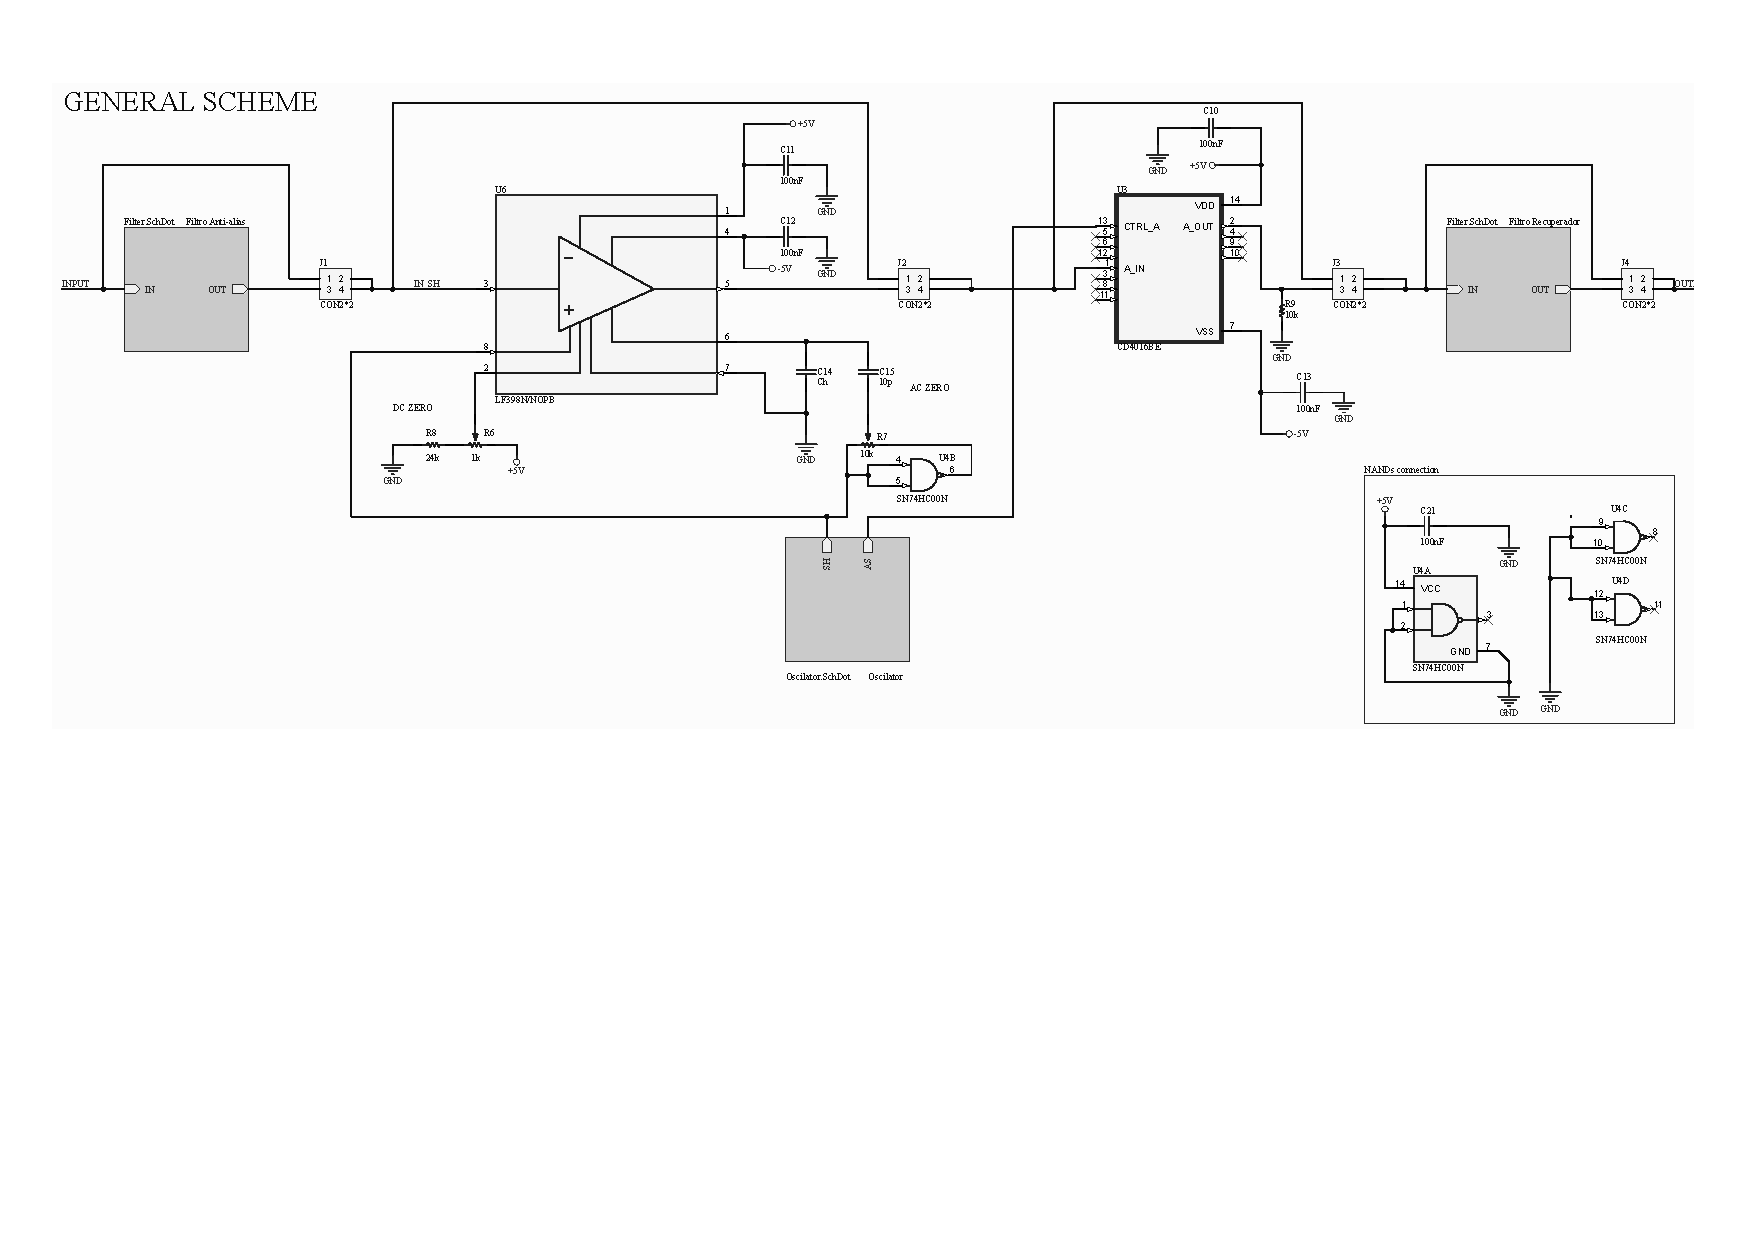
\includegraphics[width=0.9\textwidth]{Imagenes/5_PCB/General_Scheme.pdf}
	\caption{Esquemático general del sistema. Se incluyen los \textit{jumpers} de ruteo para habilitar y deshabilitar las distintas etapas de muestreo según lo requerido.}
	\label{fig:esquematico}
\end{figure}

\begin{figure}[H]
	\begin{subfigure}[c]{0.45\textwidth}
		\centering
		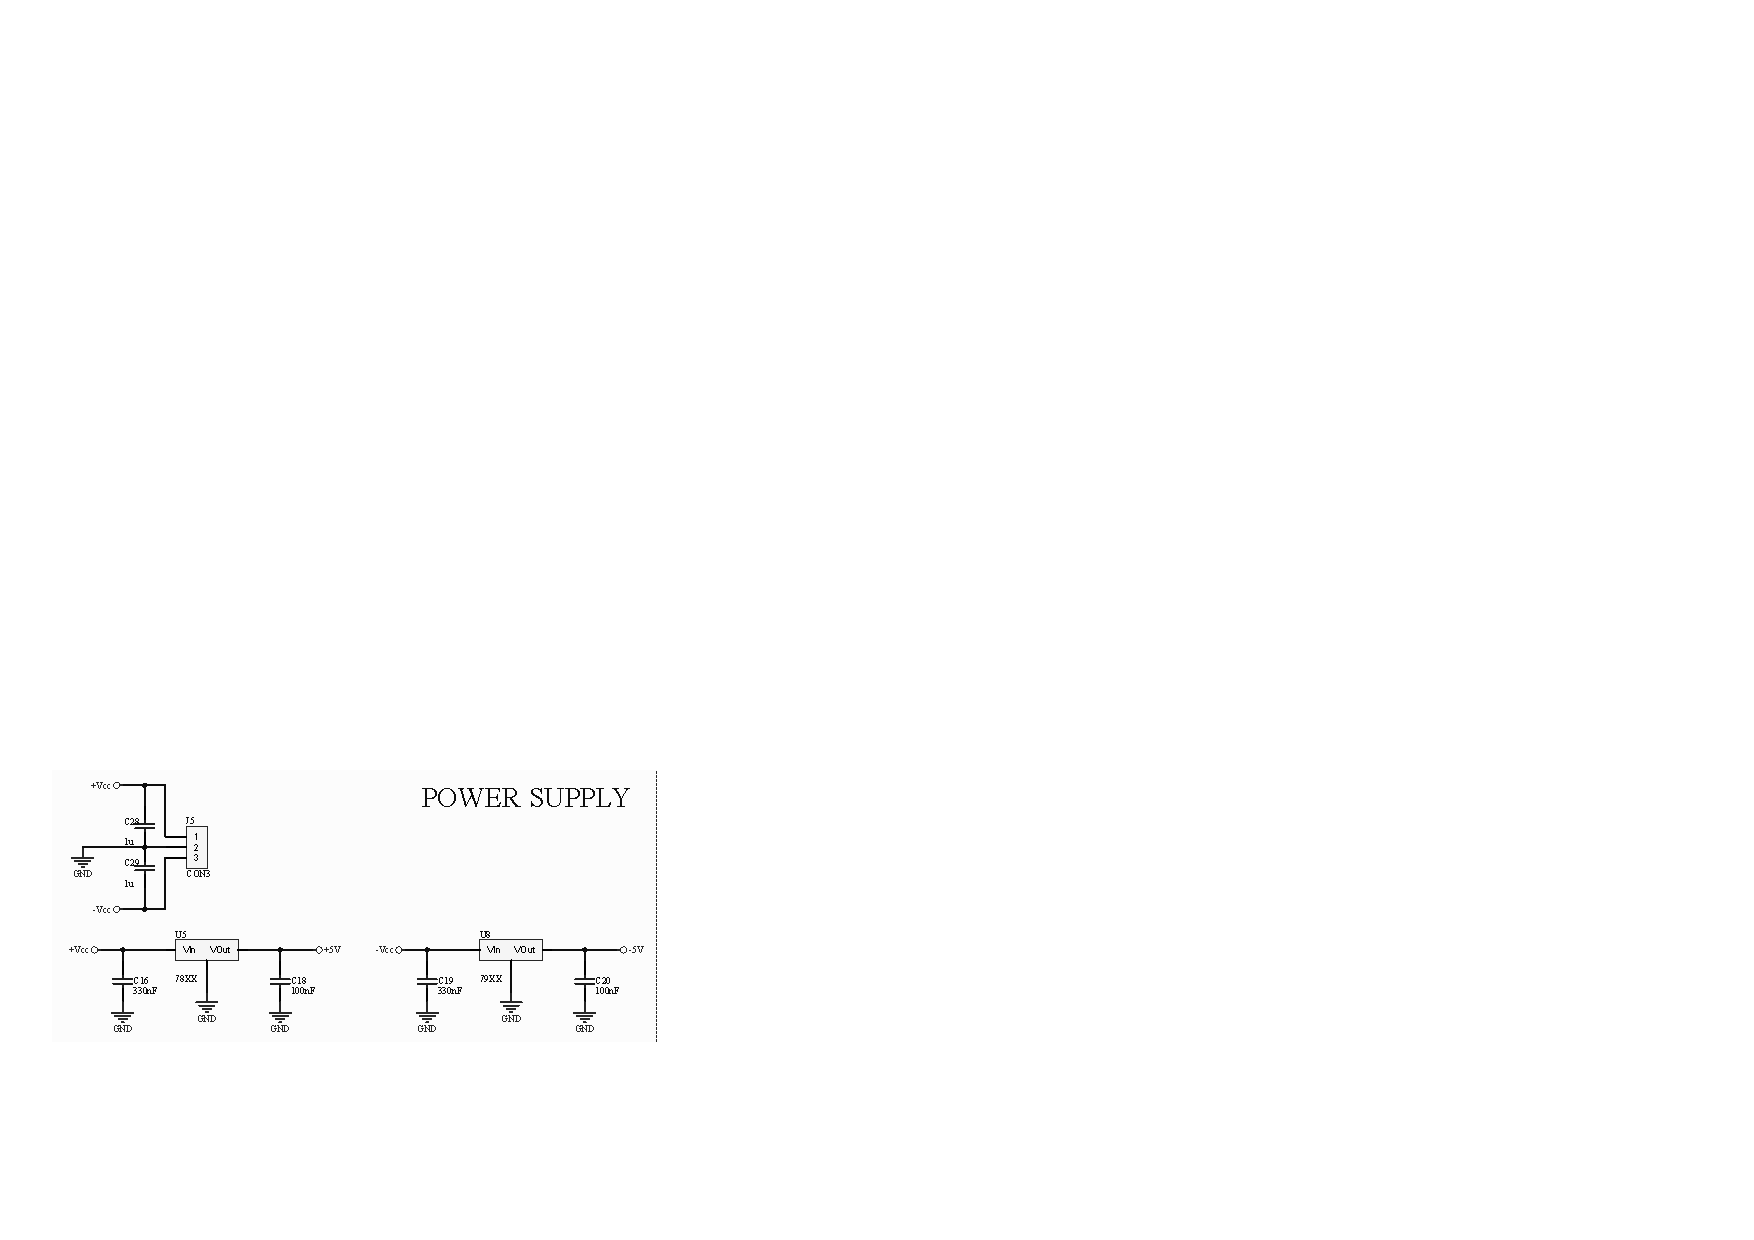
\includegraphics[width=0.9\textwidth]{Imagenes/5_PCB/Fuente_Poder.pdf}
		\caption{Esquemático referente a la alimentación de entrada.}
		\label{fig:esquematico}
	\end{subfigure}
	\hfill
	\begin{subfigure}[c]{0.45\textwidth}
		\centering
		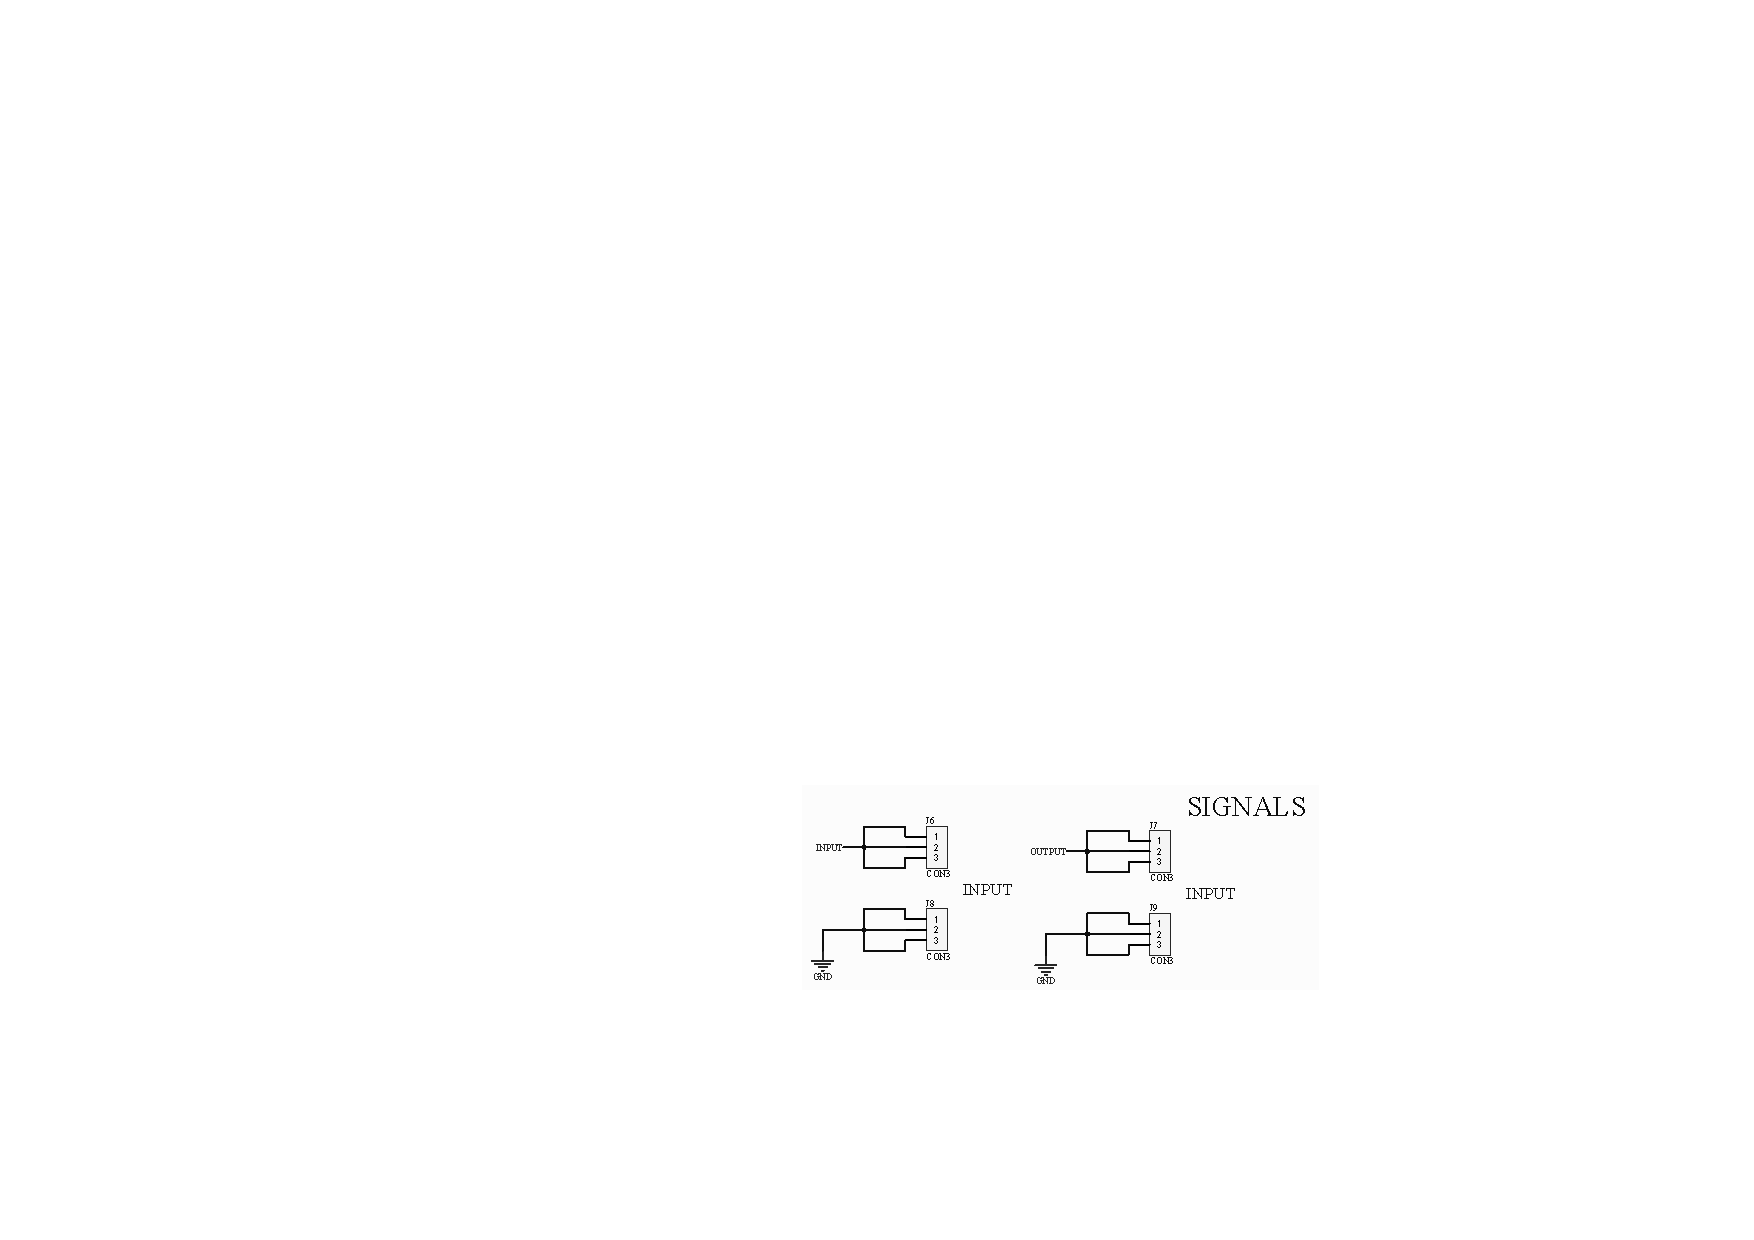
\includegraphics[width=0.9\textwidth]{Imagenes/5_PCB/Señales.pdf}
		\caption{Esquemático referente a la entrada de señales dadas por las diferentes etapas.}
		\label{fig:esquematico}
	\end{subfigure}
\end{figure}

\begin{figure}[H]
	\begin{subfigure}[c]{0.45\textwidth}
		\centering
		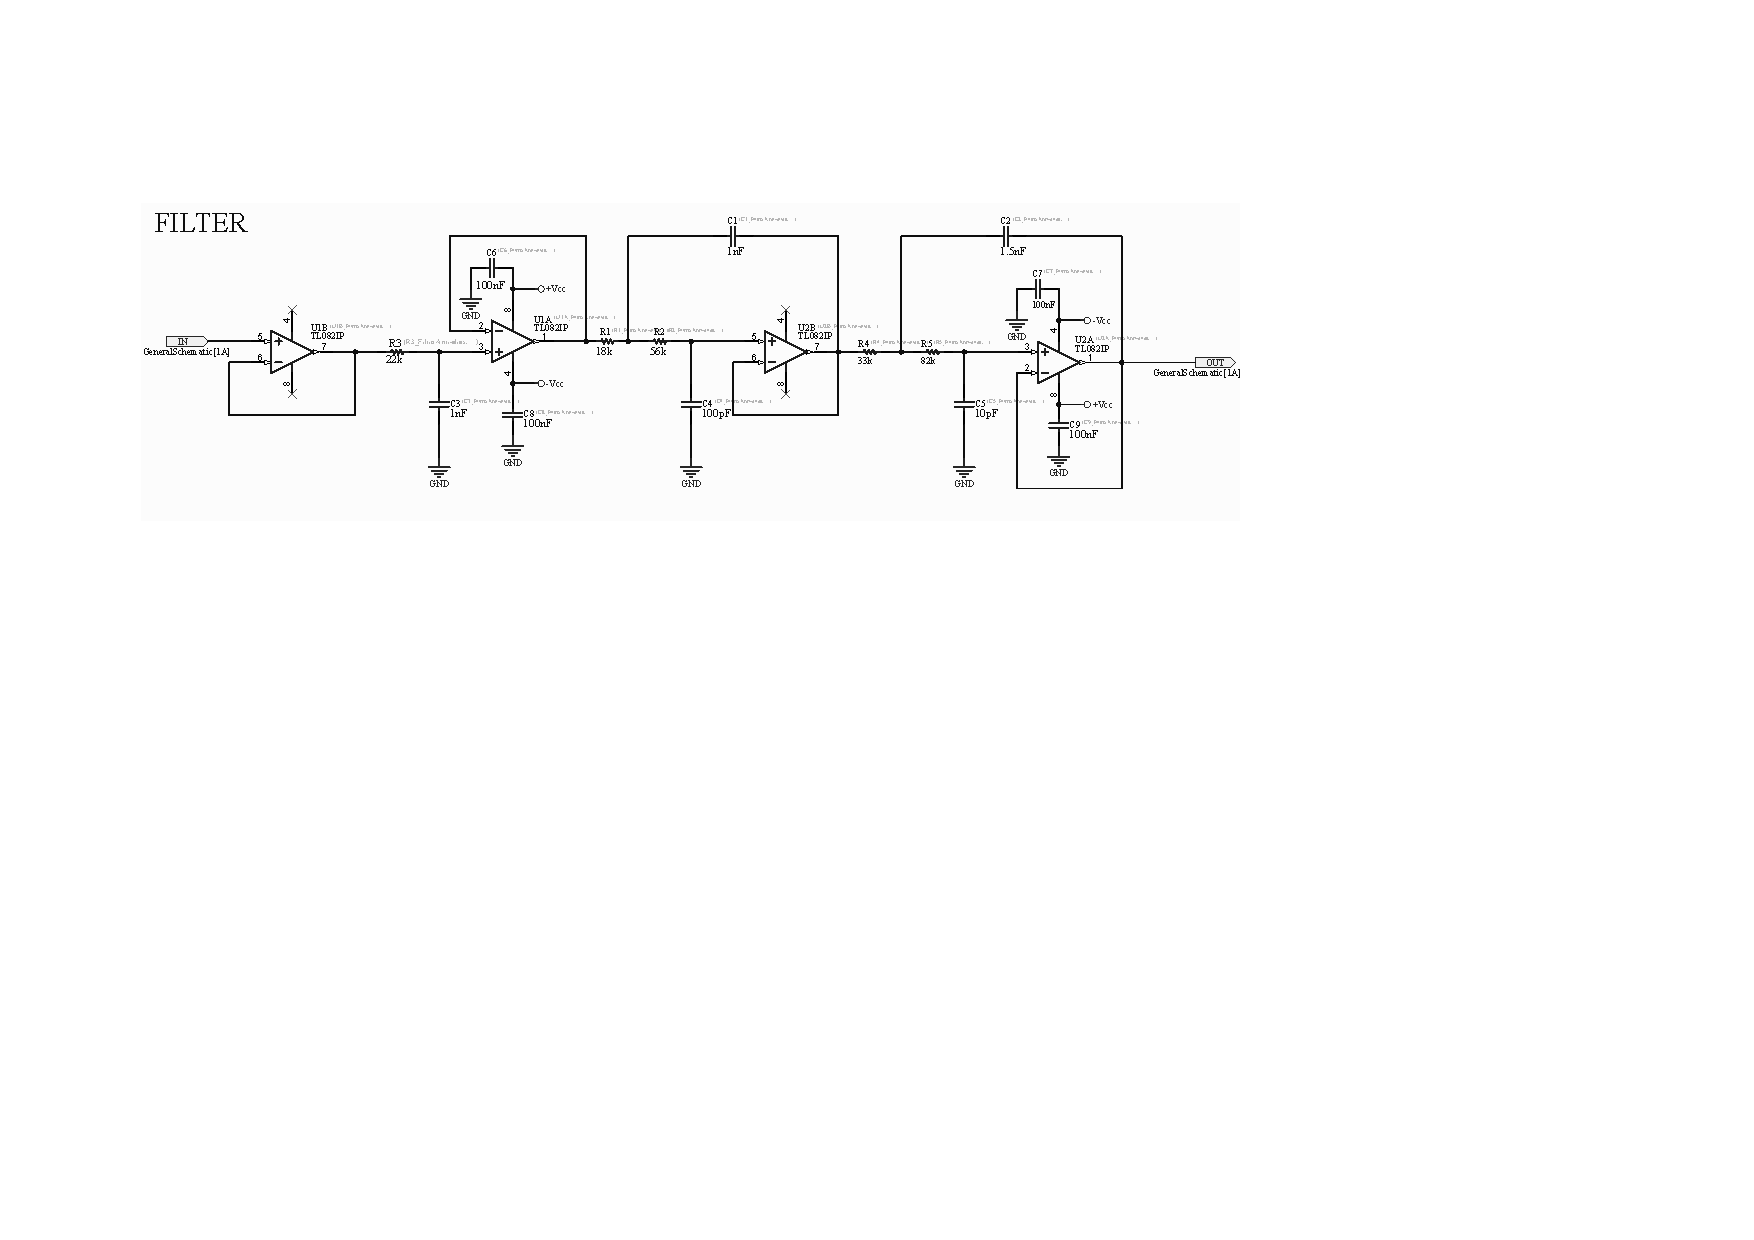
\includegraphics[width=0.9\textwidth]{Imagenes/5_PCB/Filtro_Scheme.pdf}
		\caption{Esquemático referente a el filtro anti-aliasing y recuperador.}
		\label{fig:esquematico}
	\end{subfigure}
	\hfill
	\begin{subfigure}[c]{0.45\textwidth}
		\centering
		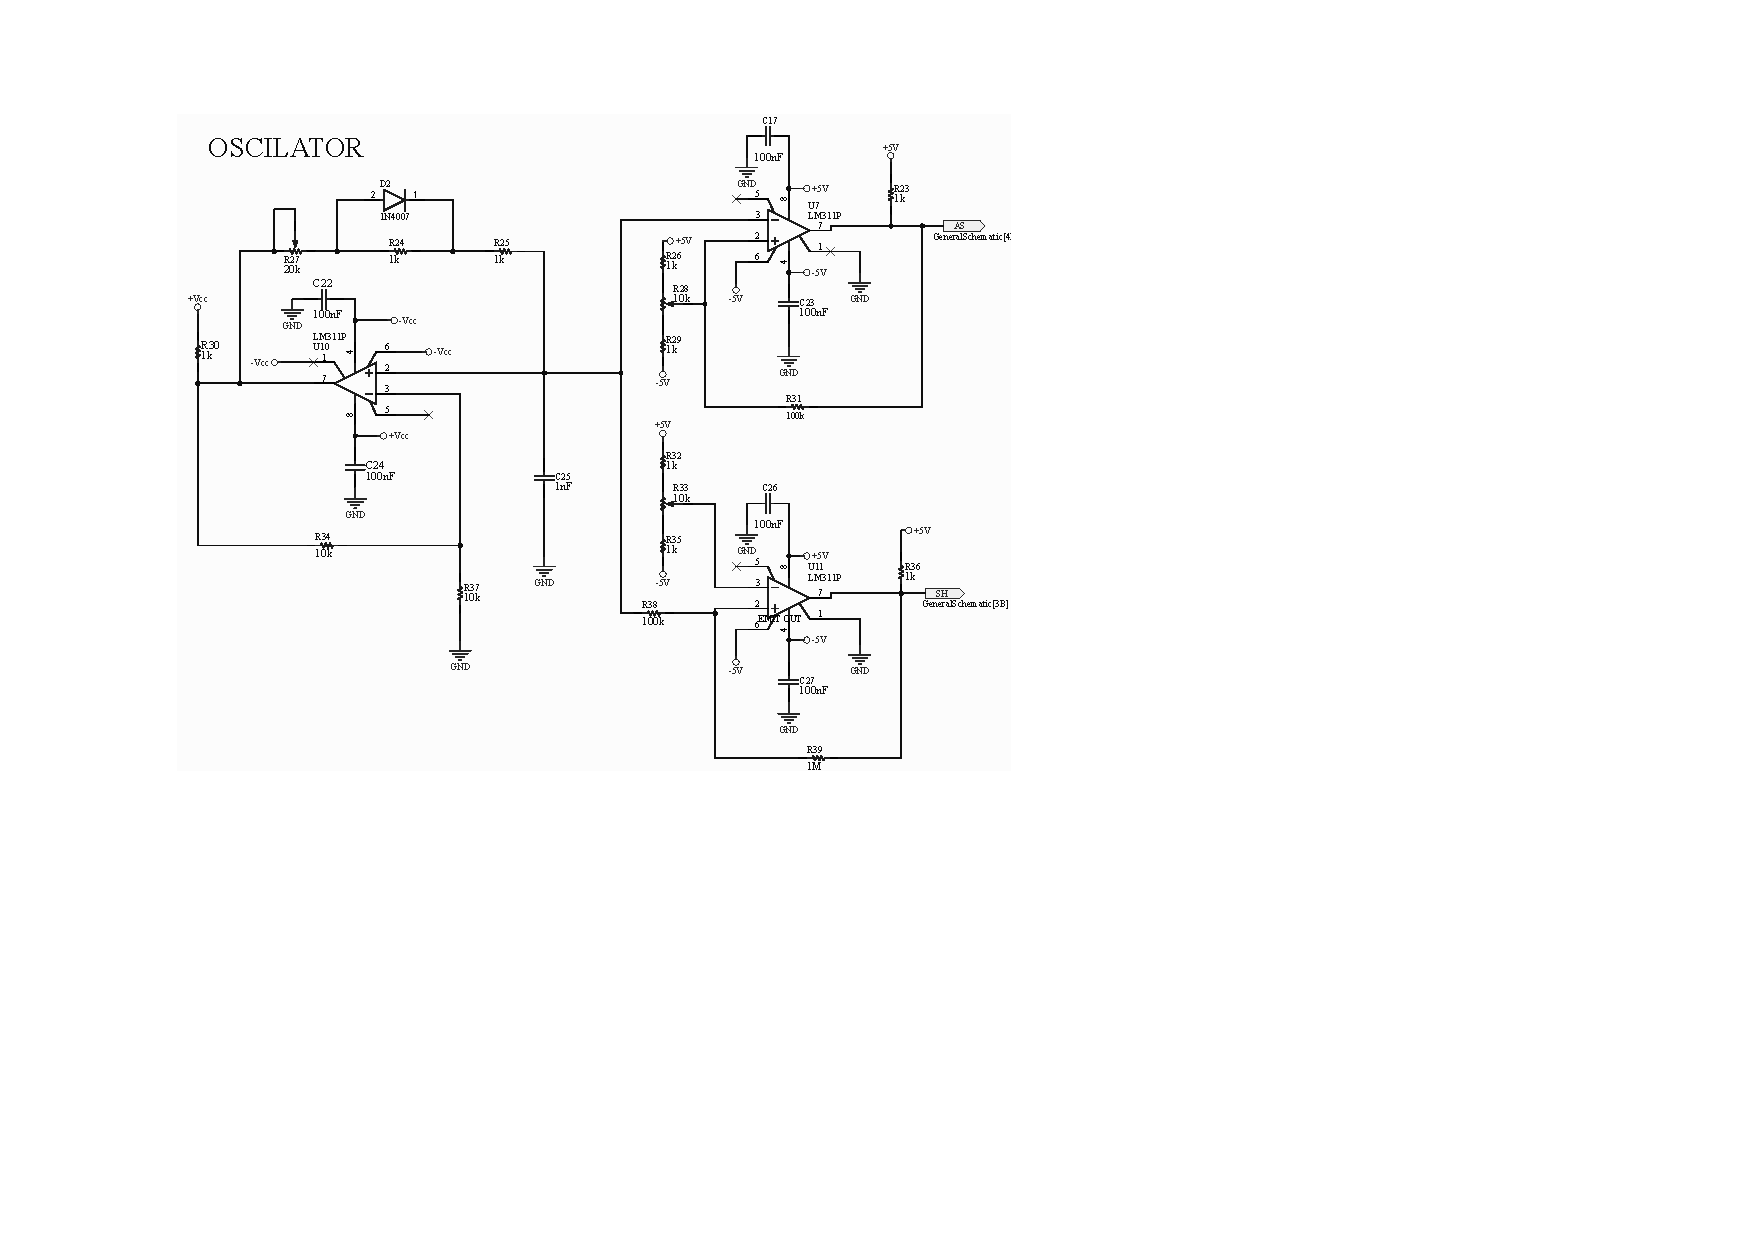
\includegraphics[width=0.9\textwidth]{Imagenes/5_PCB/Oscilador_Scheme.pdf}
		\caption{Esquemático referente al oscilador utilizado.}
		\label{fig:esquematico}
	\end{subfigure}
\end{figure}
\newpage
\subsubsection{Layout}
\begin{figure}[H]
	\begin{subfigure}[c]{0.5\textwidth}
		\centering
		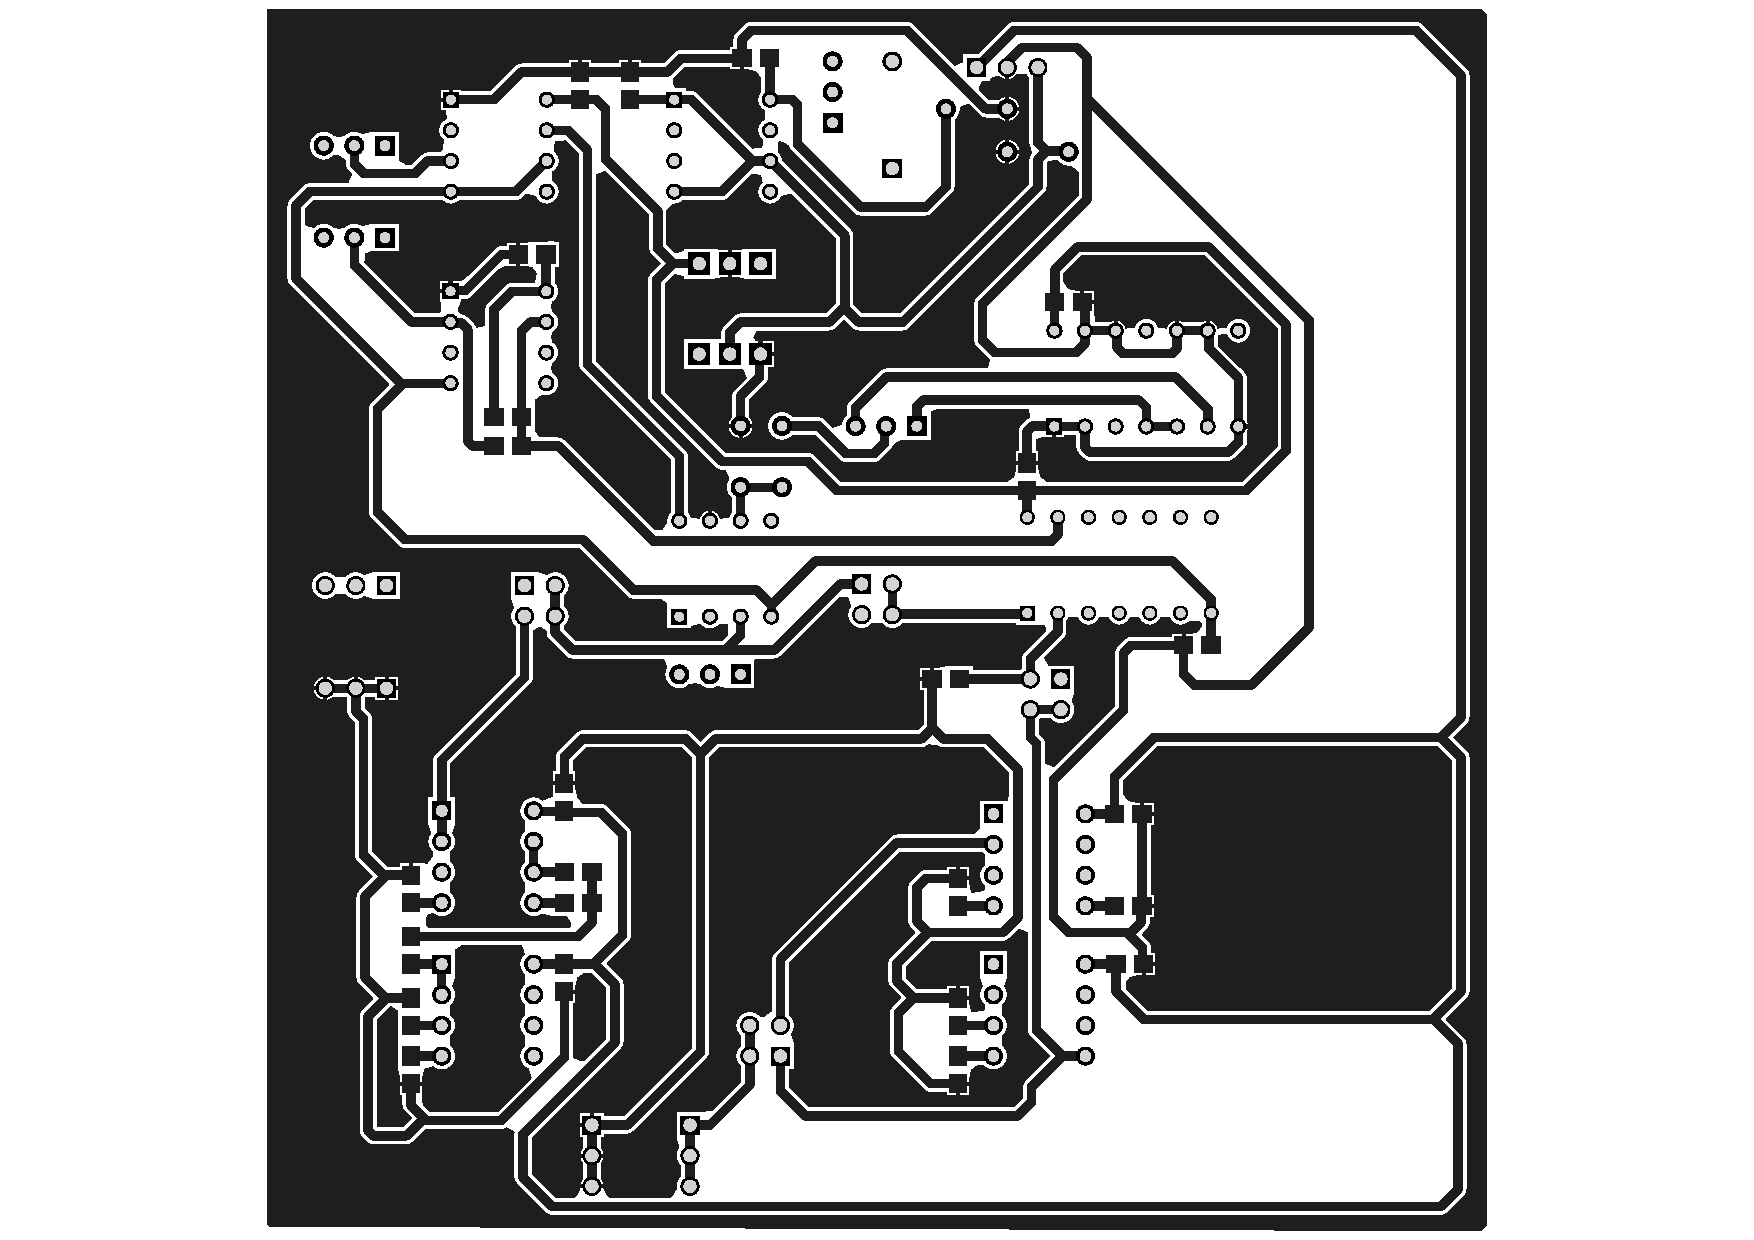
\includegraphics[width=0.95\textwidth]{Imagenes/5_PCB/Top-Layer.pdf}
		\caption{Layout referente a la parte frontal del PCB.}
		\label{fig:esquematico}
	\end{subfigure}
	\hfill
	\begin{subfigure}[c]{0.5\textwidth}
		\centering
		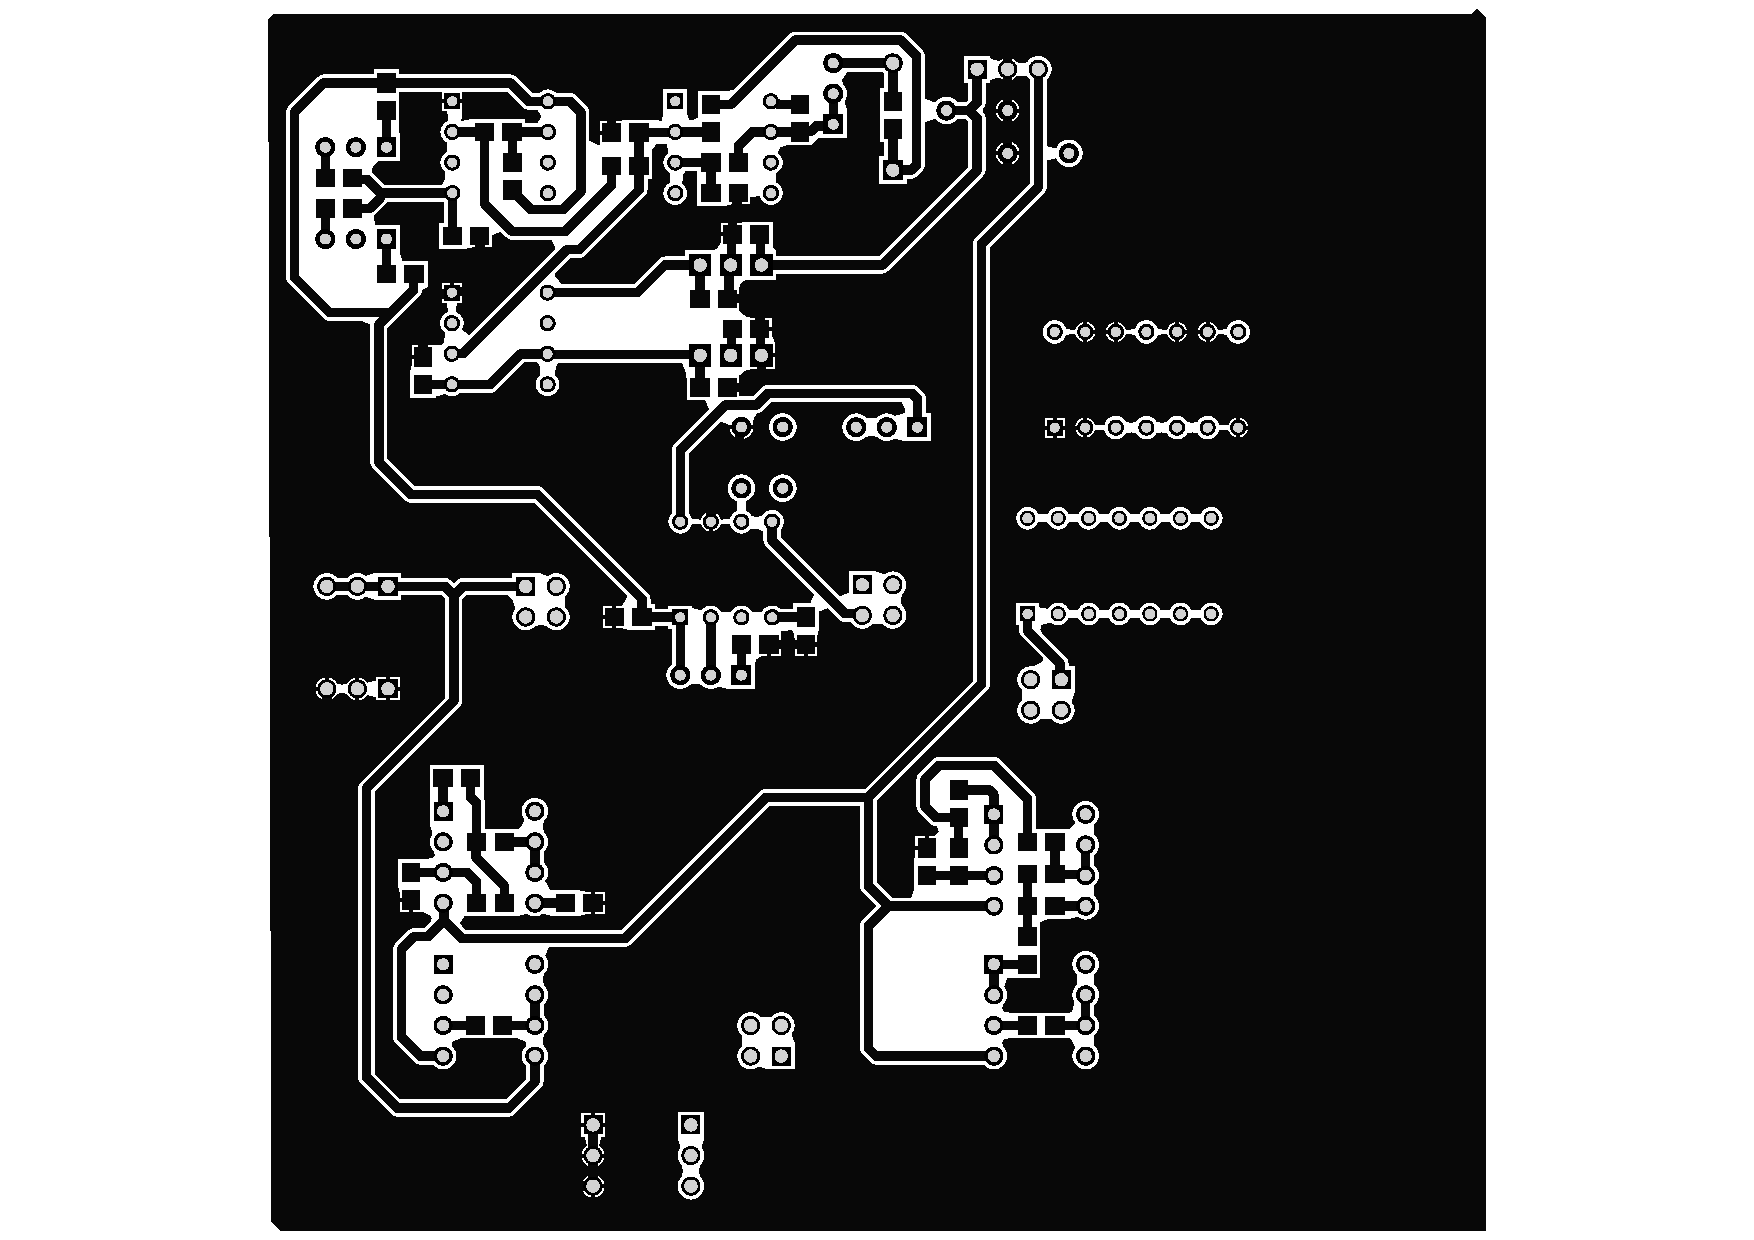
\includegraphics[width=0.95\textwidth]{Imagenes/5_PCB/Bottom-Layer.pdf}
		\caption{Layout referente a la parte trasera del PCB.}
		\label{fig:esquematico}
	\end{subfigure}
	\begin{subfigure}[c]{0.5\textwidth}
		\centering
		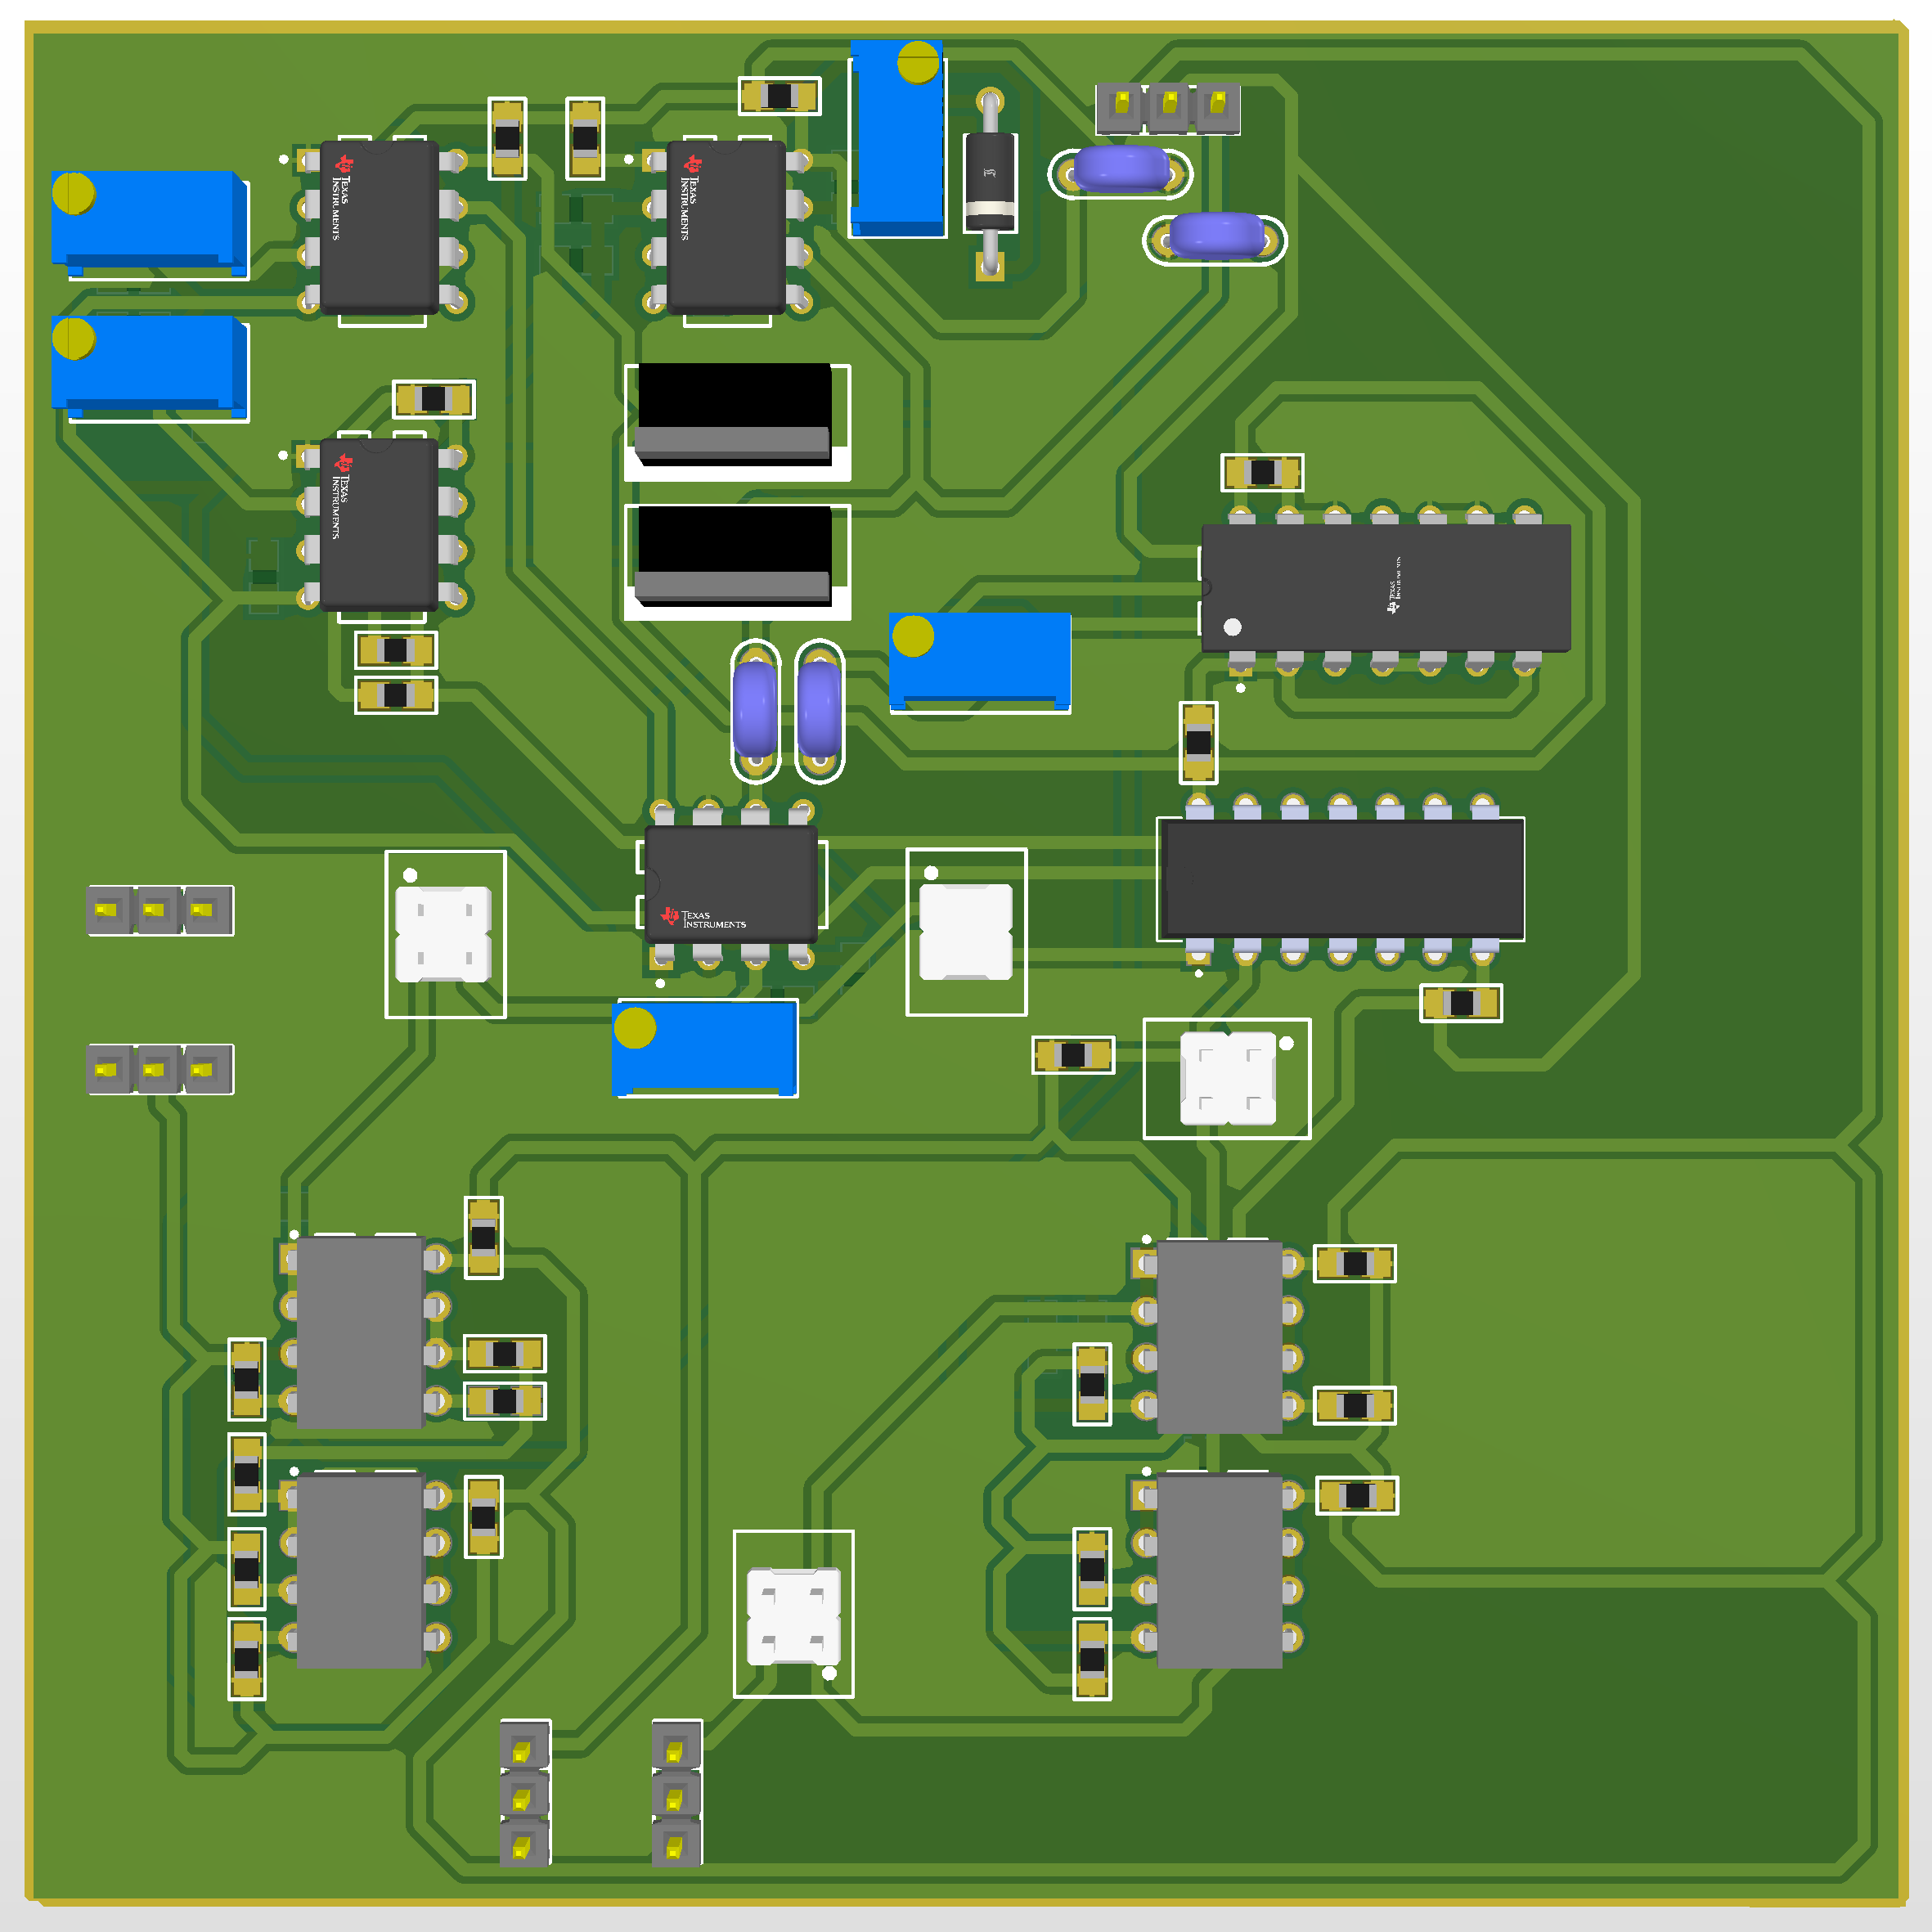
\includegraphics[width=0.65\textwidth]{Imagenes/5_PCB/PCB_Frontal.png}
		\caption{Layout referente a la parte frontal del PCB.}
		\label{fig:esquematico}
	\end{subfigure}
	\hfill
	\begin{subfigure}[c]{0.5\textwidth}
		\centering
		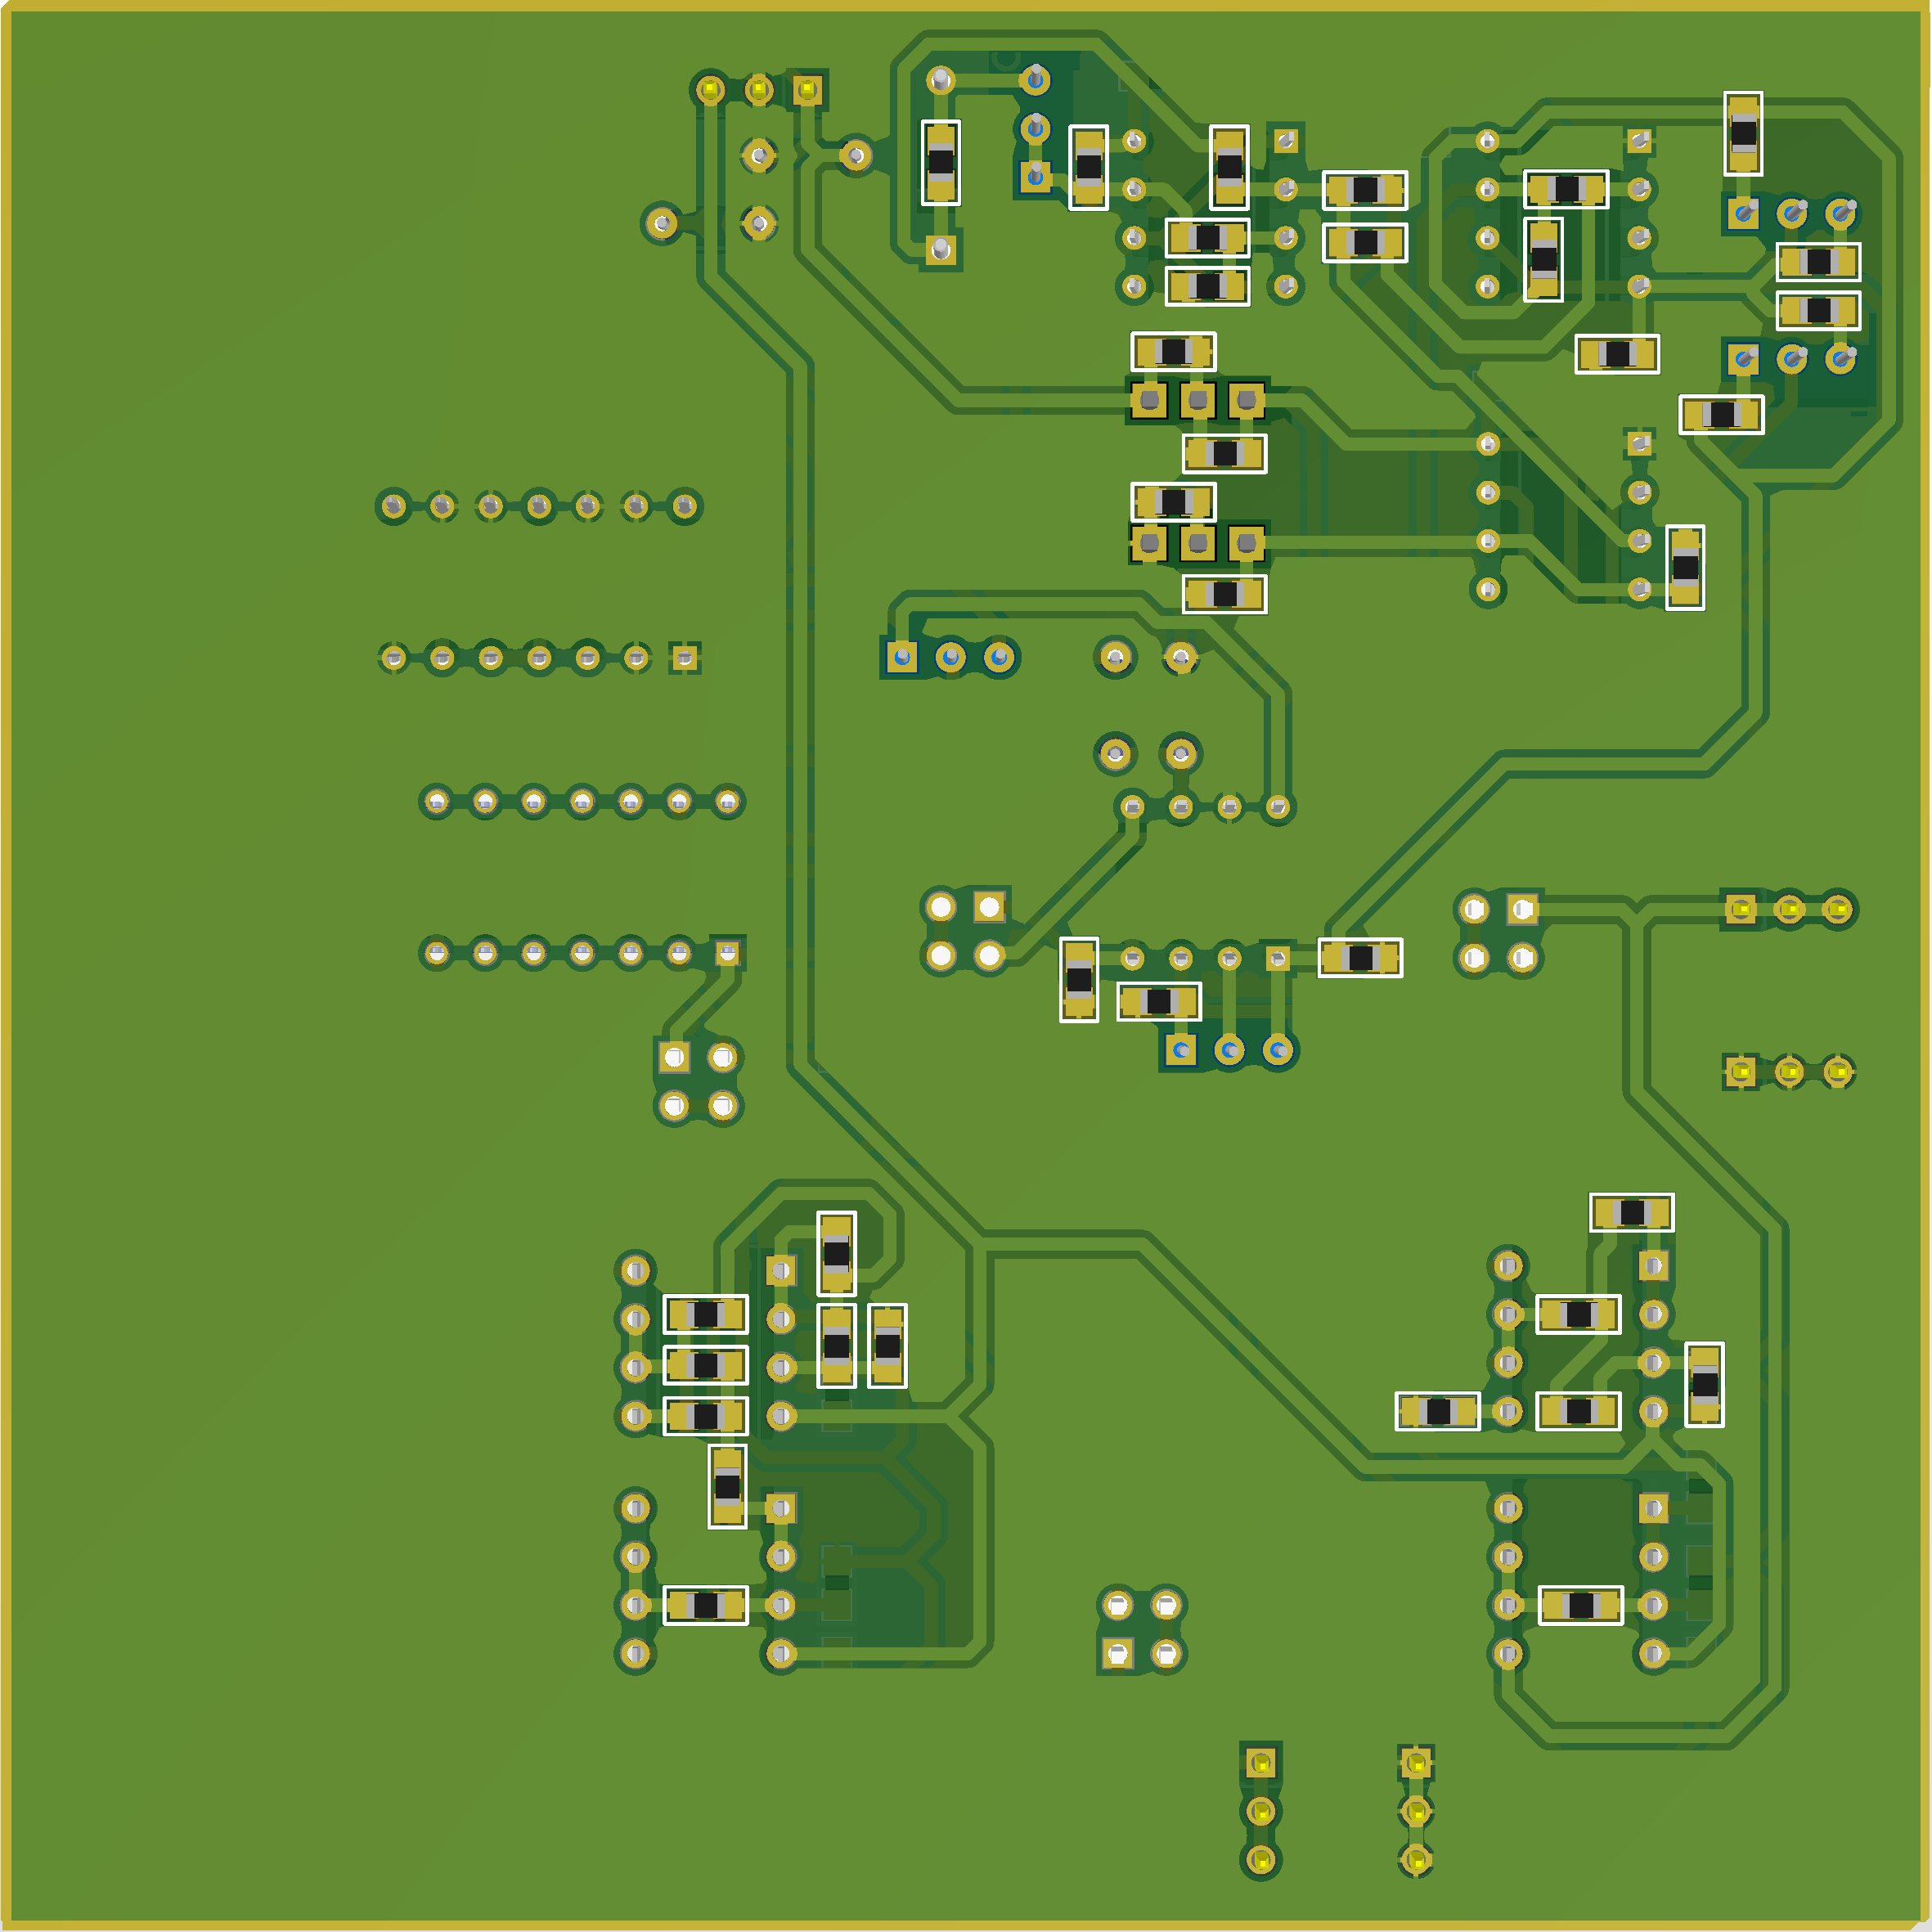
\includegraphics[width=0.65\textwidth]{Imagenes/5_PCB/PCB_Trasero.png}
		\caption{Layout referente a la parte trasera del PCB.}
		\label{fig:esquematico}
	\end{subfigure}
\end{figure}
\subsubsection{Bill of Materials (BOM)}

\begin{table}[htbp]
	\centering
	\caption{Lista de Materiales (BOM) resumida por bloques funcionales.}
	\label{tab:bom_resumido}
	\setlength{\tabcolsep}{4pt}
	\scalebox{0.75}{
	\begin{tabular}{|c|c|c|c|}
		\hline
		\textbf{Componente} & \textbf{Cant.} & \textbf{Descripción / Función} & \textbf{Designadores} \\ \hline
		\hline
		\multicolumn{4}{|c|}{\textbf{Circuitos Integrados}} \\ \hline
		TL082IP & 4 & Amplificador Operacional JFET Dual & U1, U2 (FA y FR) \\ \hline
		LM311P & 3 & Comparador de voltaje diferencial & U7, U10, U11 \\ \hline
		LF398N & 1 & Sample and Hold (S\&H) & U6 \\ \hline
		CD4016BE & 1 & Quad Bilateral Switch & U3 \\ \hline
		SN74HC00N & 1 & Compuertas NAND Quad 2-Input & U4 \\ \hline
		78XX / 79XX & 2 & Reguladores de tensión LDO (+5V, -5V) & U5, U8 \\ \hline
		\hline
		\multicolumn{4}{|c|}{\textbf{Capacitores}} \\ \hline
		100nF & 21 & Cerámicos (Desacople y filtrado general) & C6-C13, C17-C27 \\ \hline
		1nF, 1.5nF & 7 & Capacitores para diseño de filtros activos & C1-C3, C25 \\ \hline
		10pF, 100pF & 5 & Cerámicos (Compensación de fase) & C4, C5, C15 \\ \hline
		330nF, 1$\mu$F & 4 & Filtrado para reguladores de tensión & C16, C19, C28, C29 \\ \hline
		Ch & 1 & Capacitor de retención para S\&H & C14 \\ \hline
		\hline
		\multicolumn{4}{|c|}{\textbf{Resistencias}} \\ \hline
		18k$\Omega$ a 82k$\Omega$ & 10 & Precisión para topologías de filtros & R1-R5 (FA y FR) \\ \hline
		1k$\Omega$ a 1M$\Omega$ & 23 & Resistencias de pull-up, divisores y polarización general & R6-R9, R23-R39 \\ \hline
		\hline
		\multicolumn{4}{|c|}{\textbf{Conectores y Otros}} \\ \hline
		CON2x2, CON3 & 9 & Conectores tipo Header (E/S y alimentación) & J1-J9 \\ \hline
		1N4007 & 1 & Diodo rectificador & D2 \\ \hline
	\end{tabular}}
\end{table}
\newpage
\subsection{Criterios y medidas especiales tomadas durante el diseño del PCB}
El desempeño de los circuitos analógico-digitales es altamente susceptible al ruido y a las interferencias parásitas propias de la implementación física. Para asegurar la integridad de la señal y evitar que el \textit{layout} atente contra la funcionalidad del circuito, se adoptaron los siguientes criterios de diseño en Altium:

\begin{itemize}
	\item \textbf{Separación de dominios Analógico y Digital:} Las pistas correspondientes al circuito oscilador poseen flancos de subida y bajada muy abruptos. Para evitar el acoplamiento electromagnético (\textit{crosstalk}) hacia la señal de información, se ruteó la sección digital físicamente distanciada de las etapas del filtro anti-alias (FAA), el \textit{Sample and Hold} y el filtro recuperador (FR).
	
	\item \textbf{Protección del nodo de \textit{Hold} (Alta Impedancia):} El pin 6 del LF398, donde se conecta el capacitor de \textit{hold} ($C_h$), es un nodo de altísima impedancia. Para minimizar las corrientes de fuga inducidas por el sustrato del PCB (FR4), la pista que une $C_h$ con el pin 6 se diseñó con la menor longitud posible, minimizando el área expuesta para no captar ruido radiado ambiental.
	
	\item \textbf{Desacople de las líneas de alimentación:} Se dispusieron capacitores de desacople (\textit{bypass}) cerámicos, típicamente de $100\text{ nF}$, ubicados geométricamente lo más cerca posible de los pines de alimentación ($\pm10\text{V}$ y $\pm5\text{V}$) de todos los circuitos integrados (TL082, LM311, LF398, CD4016). Esto garantiza una reserva local de carga frente a los picos de corriente exigidos durante la conmutación rápida de la llave analógica y los comparadores.
	
	\item \textbf{Manejo del plano de masa (GND):} Se prestó especial atención al retorno de las corrientes. Se implementó un plano de masa robusto (o ruteo en estrella) para evitar bucles de masa (\textit{ground loops}), asegurando que las corrientes de conmutación de la etapa digital no compartan el mismo camino de retorno que las señales analógicas de precisión, lo cual introduciría ruido en la referencia de los filtros de Chebyshev.
\end{itemize}